\documentclass[12pt]{article}


\usepackage{tabularx}
\usepackage[table]{xcolor}
\usepackage{multirow}

\usepackage{tikz} 
\usetikzlibrary{automata} 
\usetikzlibrary{positioning} 
\usetikzlibrary{arrows} 

\tikzset{node distance=2.5cm, 
every state/.style={ % Sets the properties for each state
semithick,
fill=gray!10},
initial text={}, % No label on start arrow
double distance=2pt, % Adjust appearance of accept states
every edge/.style={ % Sets the properties for each transition
draw,
->, % Makes edges directed with bold arrowheads
auto,
semithick}}
\let\epsilon\varepsilon

\usepackage{amsmath, amssymb}
\usepackage{mathtools}

\usepackage[most]{tcolorbox}

\tcbset{
    frame code={}
    center title,
    left=10pt,
    right=10pt,
    top=10pt,
    bottom=10pt,
    colback=gray!5,
    colframe=gray,
    width=\dimexpr\textwidth\relax,
    enlarge left by=0mm,
    boxsep=5pt,
    arc=0pt,outer arc=0pt,
}

\usepackage[margin=1.1in,footskip=.25in]{geometry}

\renewcommand{\baselinestretch}{1.3} 


\begin{document}

\section{Introduction}

\subsection{finite automaton}

\textbf{finite automaton} is used in :

\begin{itemize}
	\item text processing
	\item compilers
	\item hardware design
\end{itemize}

\subsection{context-free grammar}

\textbf{context-free grammar} is used in :

\begin{itemize}
	\item programming languages
	\item artificial intelligence
\end{itemize}


\subsection{set}

a \textbf{set} is a group of objects represented as a unit .

\noindent
The objects in a set are called its \textbf{elements} or \textbf{members} .

\noindent
a set with one member is called the \textbf{empty set} .

\noindent
a set with one member is sometimes called a \textbf{singleton set} .

\noindent
a set with two members is called an \textbf{unordered pair} .



\subsection{Sequence and Tuples}

a \textbf{sequence} of objects is a list of these objects in some order .

\noindent
we usually designate a sequence by writing the list within parentheses . For example : $
( 7 , 21 , 57 )
$

\noindent
The order doesn't matter in a set, but in a sequence it does .

\noindent
repetition does matter in sequence, but it doesn't matter in a set .

\noindent
Finite sequences often are called \textbf{tuples} .

\noindent
a sequence with k elements is a \textbf{k-tuple} .

\noindent
a 2-tuple is also called an \textbf{ordered pair} .


\subsection{alphabet}

\textbf{alphabet} is a finite non-empty set of objects called symbols .


\subsection{string over an alphabet}

a string over an alphabet is a finite sequence of symbols from that alphabet .

\subsection{language}

a language is a set of strings .


\subsection{Summary}

\begin{itemize}
	\item [\textbf{Alphabet}] a finite non-empty set of objects called symbols 
	\item [\textbf{Empty set}] The set with no members 
	\item [\textbf{Empty string}] The string of length zero 
	\item [\textbf{k-tuple}] ordered list of k objects 
	\item [\textbf{Language}] a set of strings 
	\item [\textbf{Member}] an object in a set 
	\item [\textbf{sequence}] ordered list of objects 
	\item [\textbf{ordered pair}] sequence of two elements 
	\item [\textbf{unordered pair}] a set with two membes 
	\item [\textbf{set}] a group of objects 
	\item [\textbf{string}] a finite list of symbols from an alphabet
	\item [\textbf{symbol}] a member of an alphabet
\end{itemize}



\section{Regular Languages}


\subsection{Formal Definition Of a Finite Automaton}

The formal definition says that a finite automaton is a list of these five objects :

\begin{enumerate}
	\item set of states
	\item input alphabet
	\item rules for moving
	\item start state
	\item accept states
\end{enumerate}


\begin{tcolorbox}
a \textbf{finite automaton} is a 5-tuple $( Q, \Sigma , \delta , q_{0} , F )$, where :
\begin{enumerate}
	\item $Q$ is a finite set called the \textbf{states}
	\item $\Sigma$ is a finite set called \textbf{alphabets}
	\item $\delta : Q \times \Sigma \to Q$ is the \textbf{transition function}
	\item $q_{0} \in Q$ is the \textbf{start state}
	\item $F \subseteq Q$ is the set of \textbf{accept states}
\end{enumerate}
\end{tcolorbox}

\newpage

\subsection{Example}

\begin{center}
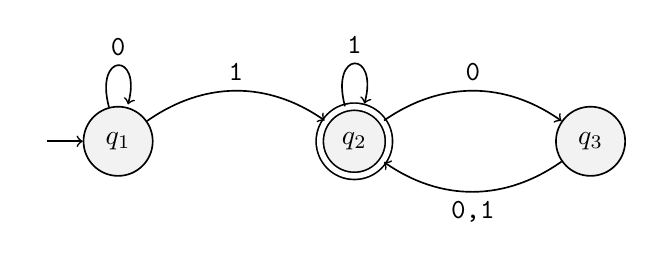
\begin{tikzpicture}
\node[state, initial] (q1) at (0,0) {$q_1$};
\node[state, accepting] (q2) at (3,0) {$q_2$};
\node[state] (q3) at (6,0) {$q_3$};
\draw (q1) edge[loop above] node {\tt 0} (q1) ;
\draw (q1) edge[bend left=35] node {\tt 1} (q2) ;
\draw (q2) edge[loop above] node {\tt 1} (q2) ;
\draw (q2) edge[bend left=35] node {\tt 0} (q3) ;
\draw (q3) edge[bend left=35] node {\tt 0,1} (q2);
\end{tikzpicture}
\end{center}

We can describe the finite automata M formally writing $M = (Q , \Sigma , \delta , q_{1} , F)$ , where :

\begin{enumerate}
	\item $Q = \{ q_{1} , q_{2} , q_{3} \}$
	\item $\Sigma = \{ 0 , 1 \}$
	\item $\delta$ is described as :
	\begin{center}
	\begin{tabular}{ r | c  c  } 
	\multicolumn{3}{ c }{Transition Table} \\
	               & 0 & 1   \\
	\hline
	$q_{1}$ & $q_{1}$ & $q_{2}$   \\
	$q_{2}$ & $q_{3}$ & $q_{2}$   \\
	$q_{3}$ & $q_{2}$ & $q_{2}$   \\
	\end{tabular}
	\end{center}
	\item $q_{1}$ is the start state
	\item $F = \{ q_{2} \}$
\end{enumerate}

\noindent
if $A$ is the set of all strings that machine $M$ accepts, we say that $A$ is the \textbf{language of machine M} and write $L(M) = A$ . We also say that \textbf{M recognizes A} of \textbf{M accepts A} .

\noindent
a machine may accept several string, but it always recognizes only one language .

\noindent
if the machine accepts no strings, it still recognized one languages, the empty language $\emptyset$ .



\newpage

\subsection{Example}

You can see the state diagram of the two-state finite automaton M :

\begin{center}
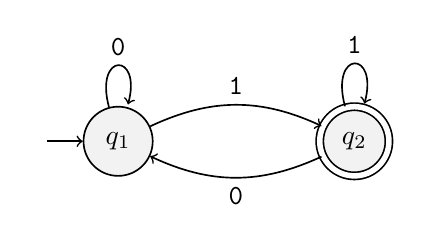
\begin{tikzpicture}
\node[state, initial] (q1) at (0,0) {$q_1$};
\node[state, accepting] (q2) at (3,0) {$q_2$};
\draw (q1) edge[loop above] node {\tt 0} (q1) ;
\draw (q1) edge[bend left=25] node {\tt 1} (q2) ;
\draw (q2) edge[loop above] node {\tt 1} (q2) ;
\draw (q2) edge[bend left=25] node {\tt 0} (q1) ;
\end{tikzpicture}
\end{center}


in the formal description , $M = ( Q , \Sigma , \delta , q_{1} , F )$
, where : 

\begin{enumerate}
	\item $Q = \{ q_{1} , q_{2} \}$
	\item $\Sigma = \{ 0 , 1 \}$
	\item $\delta$ is described as :
	\begin{center}
	\begin{tabular}{ r | c  c  } 
	\multicolumn{3}{ c }{Transition Table} \\
	               & 0 & 1   \\
	\hline
	$q_{1}$ & $q_{1}$ & $q_{2}$   \\
	$q_{2}$ & $q_{1}$ & $q_{2}$   \\
	\end{tabular}
	\end{center}
	\item $q_{1}$ is the start state
	\item $F = \{ q_{2} \}$
\end{enumerate}

\begin{tcolorbox}
\begin{itemize}
	\item after trying a few examples, you would see that M accepts all strings that end in $1$ . Thus 
	$$
	L(M) = \{ w \:\: | \:\: w \:\: ends \:\: in \:\: a \:\: 1 \}
	$$
\end{itemize}
\end{tcolorbox}

\begin{tcolorbox}
\begin{itemize}
	\item Note that the machine accepts all strings that leave it in an accept state when it has finished reading .
\end{itemize}
\end{tcolorbox}


\subsection{Example}

in the following Machine we just \textbf{change the position of  accepting state} .

\begin{center}
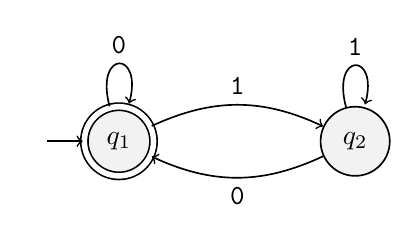
\begin{tikzpicture}
\node[state , initial, accepting ] (q1) at (0,0) {$q_1$};
\node[state ] (q2) at (3,0) {$q_2$};
\draw (q1) edge[loop above] node {\tt 0} (q1) ;
\draw (q1) edge[bend left=25] node {\tt 1} (q2) ;
\draw (q2) edge[loop above] node {\tt 1} (q2) ;
\draw (q2) edge[bend left=25] node {\tt 0} (q1) ;
\end{tikzpicture}
\end{center}

\begin{tcolorbox}
\begin{itemize}
	\item the language of Machine M is :
	$$
	L(M) = \{ w \:\: | \:\: w \:\: is \:\: the \:\: empty \:\: string \:\: \epsilon \:\: or \:\: ends \:\: in \:\: 0 \}
	$$
\end{itemize}
\end{tcolorbox}



\subsection{Formal Definition Of Computation}

Let $M=(Q , \Sigma , \delta , q_{0} , F)$ be a finite automaton and let $w = w_{1}w_{2} \dots w_{n}$ be a string where each $w_{i}$ is a member of the alphabet $\Sigma$ . Then M \textbf{accepts} $w$ is a sequence of states $r_{0}, r_{1} , \dots , r_{n}$ in Q exists with three conditions :


\begin{enumerate}
	\item $r_{0} = q_{0}$
	\item $\delta(r_{i} , w_{i+1}) = r_{i+1}$, for $i = 0 , 1 , 2 , \dots , n-1$
	\item $r_{n} \in F$
\end{enumerate}


\begin{itemize}
	\item [Condition 1] says that the machine starts in the start state .
	\item [Condition 2] says that the machine goes from state to state according to the transition function
	\item [Condition 3] says that the machine accepts its input if it ends up in an accept state
	\item we say that M \textbf{recognize language} A if 
	$A = \{ w \:\: | \:\: M \:\: accepts \:\: w \}$
\end{itemize}



\begin{tcolorbox}
\begin{itemize}
	\item a language is called a \textbf{regular language} if some finite automaton recognizes it
\end{itemize}
\end{tcolorbox}


\subsection{Example}

construct a finite automaton to recognize all strings with an odd number of 1s ?

\noindent
The alphabet is : $\Sigma = \{ 0 , 1 \}$  


Answer :

\begin{center}
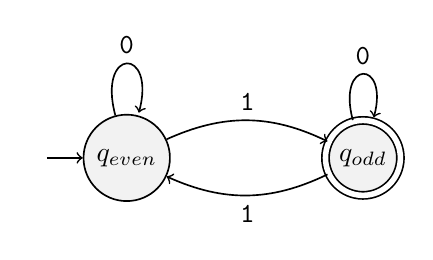
\begin{tikzpicture}
\node[state , initial ] (q1) at (0,0) {$q_{even}$};
\node[state , accepting] (q2) at (3,0) {$q_{odd}$};
\draw (q1) edge[loop above] node {\tt 0} (q1) ;
\draw (q1) edge[bend left=25] node {\tt 1} (q2) ;
\draw (q2) edge[loop above] node {\tt 0} (q2) ;
\draw (q2) edge[bend left=25] node {\tt 1} (q1) ;
\end{tikzpicture}
\end{center}




\subsection{Example}

design a finite automaton to recognize all strings that contain the substring 001 ?


Answer :

\begin{center}
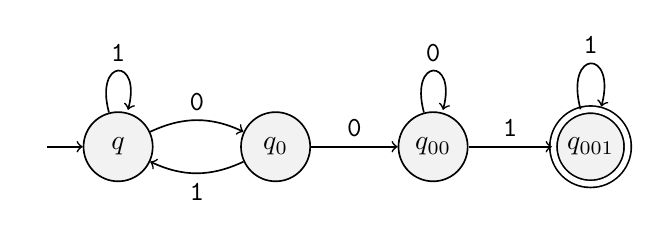
\begin{tikzpicture}
\node[state , initial ] (q0) at (0,0) {$q$};
\node[state ] (q1) at (2,0) {$q_{0}$};
\node[state ] (q2) at (4,0) {$q_{00}$};
\node[state , accepting] (q3) at (6,0) {$q_{001}$};
\draw (q0) edge[loop above] node {\tt 1} (q0) ;
\draw (q0) edge[bend left=25] node {\tt 0} (q1) ;
\draw (q1) edge[bend left=25] node {\tt 1} (q0) ;
\draw (q1) edge[] node {\tt 0} (q2) ;
\draw (q2) edge[loop above] node {\tt 0} (q2) ;
\draw (q2) edge[] node {\tt 1} (q3) ;
\draw (q3) edge[loop above] node {\tt 1} (q3) ;
\end{tikzpicture}
\end{center}


\newpage

\subsection{NonDeterminism}

when the machine is in a given state and reads the next input symbol , we know that the next state will be | it is determined . We call this \textbf{deterministic} computation .

\noindent
in a \textbf{nondeterministic} machine , several choices may exist for the next state at any point .


\subsection{DFA vs. NFA}

The difference between a deterministic finite automaton, abbreviatedDFA,
and a nondeterministic finite automaton, abbreviatedNFA :

\begin{itemize}
	\item  every state of aDFAalways has exactly one exiting transition arrow
for each symbol in the alphabet. In an NFA , a state may have zero , one , or many
exiting arrows for each alphabet symbol.
	\item in a DFA , labels on the transition arrows are symbols from the alphabet. an NFA may have arrows
labeled with members of the alphabet or $\epsilon$ . Zero , one , or many arrows may exit
from each state with the label $\epsilon$ .
\end{itemize}


\subsection{How does an NFA compute ?}

Suppose that we are running an NFA on an input
string and come to a state with multiple ways to proceed.
After reading
that symbol, the machine splits into multiple copies of itself and follows all the
possibilities in parallel. Each copy of the machine takes one of the possible ways
to proceed and continues as before. If there are subsequent choices, the machine
splits again. If the next input symbol doesn’t appear on any of the arrows exiting
the state occupied by a copy of the machine, that copy of the machine dies, along
with the branch of the computation associated with it. Finally, if any one of these
copies of the machine is in an accept state at the end of the input, the NFA accepts
the input string.
If a state with an $\epsilon$ symbol on an exiting arrow is encountered, something
similar happens.
Nondeterminism may be viewed as a kind of parallel computation wherein
multiple independent “processes” or “threads” can be running concurrently.



\newpage

\subsection{Example}

design a NFA accepts all strings of the form $0^{k}$ where k is multiple of 2 or 3 .


\begin{center}
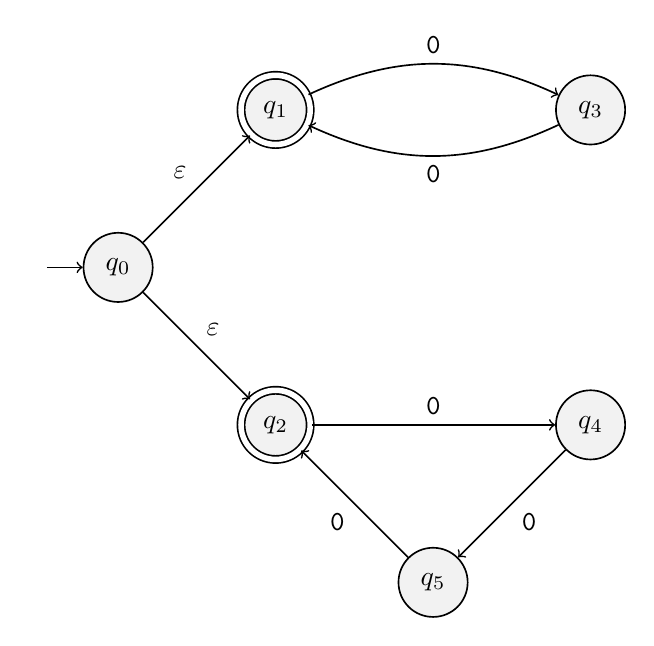
\begin{tikzpicture}
\node[state , initial ] (q0) at (0,0) {$q_{0}$};
\node[state , accepting] (q1) at (2,2) {$q_{1}$};
\node[state , accepting] (q2) at (2,-2) {$q_{2}$};
\node[state ] (q3) at (6,2) {$q_{3}$};
\node[state ] (q4) at (6,-2) {$q_{4}$};
\node[state ] (q5) at (4,-4) {$q_{5}$};
\draw (q0) edge[] node {\tt $\epsilon$} (q1) ;
\draw (q0) edge[] node {\tt $\epsilon$} (q2) ;
\draw (q1) edge[bend left=25] node {\tt 0} (q3) ;
\draw (q3) edge[bend left=25] node {\tt 0} (q1) ;
\draw (q2) edge[] node {\tt 0} (q4) ;
\draw (q4) edge[] node {\tt 0} (q5) ;
\draw (q5) edge[] node {\tt 0} (q2) ;
\end{tikzpicture}
\end{center}





\subsection{Formal Definition of a Nondeterministic Finite Automaton}


The formal definition of a nondeterministic finite automaton is similar to that of
a deterministic finite automaton . Both have states , an input alphabet , a transition
function, a start state, and a collection of accept states. However, they differ in
one essential way: in the type of transition function. In a DFA , the transition
function takes a state and an input symbol and produces the next state. In an
NFA , the transition function takes a state and an input symbol
or the empty string
and produces the set of possible next states.
For any set $Q$ we write $P(Q)$ to be
the collection of all subsets of $Q$.
Here $P(Q)$ is called the power set of $Q$.
For any
alphabet $\Sigma$ we write $\Sigma_{\epsilon}$ to be $\Sigma \cup \{ \epsilon \}$.



\begin{tcolorbox}
a  \textbf{nondeterministic finite automaton} is a 5-tuple $( Q , \Sigma , \delta , q_{0} , F )$ where :
\begin{enumerate}
	\item $Q$ is a finite set of states
	\item $\Sigma$ is a finite alphabet
	\item $\delta : Q \times \Sigma_{\epsilon} \to P(Q)$ is the transition function
	\item $q_{0} \in Q$ is the start state
	\item $F \subseteq Q$ is the set of accept states
\end{enumerate}
\end{tcolorbox}



\subsection{Example}

Suppose the following NFA :

\begin{center}
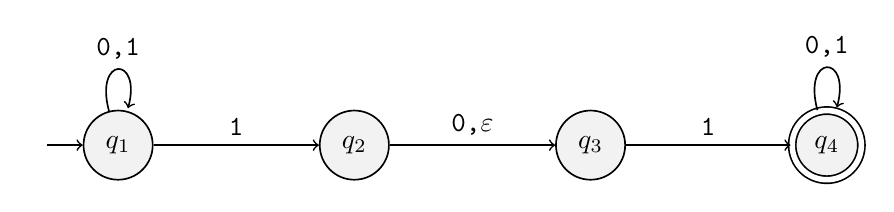
\begin{tikzpicture}
\node[state , initial ] (q0) at (0,0) {$q_{1}$};
\node[state ] (q1) at (3,0) {$q_{2}$};
\node[state ] (q2) at (6,0) {$q_{3}$};
\node[state , accepting] (q3) at (9,0) {$q_{4}$};
\draw (q0) edge[loop above] node {\tt 0,1} (q0) ;
\draw (q0) edge[] node {\tt 1} (q1) ;
\draw (q1) edge[] node {\tt 0,$\epsilon$} (q2) ;
\draw (q2) edge[] node {\tt 1} (q3) ;
\draw (q3) edge[loop above] node {\tt 0,1} (q3) ;
\end{tikzpicture}
\end{center}

The formal description of this NFA is $( Q , \Sigma , \delta , q_{1} , F)$ , where :

\begin{enumerate}
	\item $Q = \{ q_{1} , q_{2} , q_{3} , q_{4}  \}$
	\item $\Sigma = \{ 0 , 1 \}$
	\item $\delta$ is described as :
	\begin{center}
	\begin{tabular}{ r | c  c  c  } 
	\multicolumn{3}{ c }{Transition Table} \\
	               & 0 & 1 & $\epsilon$   \\
	\hline
	$q_{1}$ & $\{q_{1}\}$ & $\{q_{1} , q_{2}\}$ & $\emptyset$   \\
	$q_{2}$ & $\{q_{3}\}$ & $\emptyset$ & $\{q_{3}\}$  \\
	$q_{3}$ & $\emptyset$ & $\{q_{4}\}$ & $\emptyset$  \\
	$q_{4}$ & $\{q_{4}\}$ & $\{q_{4}\}$ & $\emptyset$  \\
	\end{tabular}
	\end{center}
	\item $q_{1}$ is the start state
	\item $F = \{ q_{4} \}$
\end{enumerate}



\subsection{Theorem}

\begin{tcolorbox}
\begin{itemize}
	\item every nondeterministic finite automaton has an equivalent deterministic finite automaton .
\end{itemize}
\end{tcolorbox}



\begin{tcolorbox}
\begin{itemize}
	\item above Theorm state that every NFA can be converted into an equivalent DFA . Thus nondeterministic finite automata give an alternative way of characterizing the regular languages . 
\end{itemize}
\end{tcolorbox}



\begin{tcolorbox}
\begin{itemize}
	\item the result of above facts is $\to$ a language is regular if and only if some nondeterministic finite automaton recognizes it .
\end{itemize}
\end{tcolorbox}



\subsection{Regular Expressions}


the language consisting of all strings starting with a 0 or 1 followed by any number of 0s .
$$
( 0 \cup 1 ) 0^{*}
$$


\noindent
the language consisting of all possible strings of 0s and 1s .
$$
( 0 \cup 1 )^{*}
$$



\noindent
suppose $\Sigma = \{ 0 , 1 \}$ , so the language contains all strings that end in a 1 .
$$
\Sigma^{*}1
$$

\noindent
suppose $\Sigma = \{ 0 , 1 \}$ , so the language consists of all strings that start with 0 or ends with 1 .
$$
( 0\Sigma^{*} ) \cup ( \Sigma^{*}1 )
$$


\subsection{Formal Definition of a Regular Expression}


\begin{tcolorbox}
Say that R is a \textbf{regular expression} if R is :
\begin{itemize}
	\item any symbol in alphabet $\Sigma$
	\item $\epsilon$
	\item $\emptyset$
	\item $( R_{1} \cup R_{2} )$, where $R_{1}$ and $R_{2}$ are regular expressions
	\item $( R_{1} \circ R_{2} )$, where $R_{1}$ and $R_{2}$ are regular expressions
	\item $( R_{1}^{*} )$, where $R_{1}$ is a regular expression
\end{itemize}
\end{tcolorbox}


\begin{tcolorbox}
Note :
\begin{itemize}
	\item $R^{+}$ be shorthand for $RR^{*}$
	\item $R^{+} \cup \epsilon = R^{*}$
\end{itemize}
\end{tcolorbox}



\newpage

\subsection{Examples}

assume the alphabet $\Sigma = \{ 0 , 1 \}$ :

\begin{tcolorbox}
\begin{enumerate}
	\item $0^{*}10^{*}$ = $\{ w | w$ contains a single 1 $\}$
	\item $\Sigma^{*}1\Sigma^{*}$ = $\{ w | w$ has at least one 1 $\}$
	\item $\Sigma^{*}001\Sigma^{*}$ = $\{ w | w$ contains the string 001 as a substring $\}$
	\item $1^{*}(01^{+})^{*}$ = $\{ w |$ every 0 in $w$ is followed by at least one 1 $\}$
	\item $(\Sigma \Sigma)^{*}$ = $\{ w | w $ is a string of even length $\}$
	\item $(\Sigma \Sigma \Sigma)^{*}$ = $\{ w |$ the length of $w$ is a multiple of 3 $\}$
	\item 01 $\cup$ 10 = $\{ 01 , 10 \}$
	\item $0\Sigma^{*} \cup 1\Sigma^{*} \cup 0 \cup 1 $ = $\{ w | w$ starts and ends with the same symbol $\}$ 
	\item $( 0 \cup \epsilon ) 1^{*}$ = $01^{*} \cup 1^{*} $
	\item $( 0 \cup \epsilon ) ( 1 \cup \epsilon )$ = $\{$ $\epsilon$ , 0 , 1 , 01 $\}$
	\item $1^{*}\emptyset$ = $\emptyset$
	\item $\emptyset^{*}$ = $\{ \epsilon \}$
\end{enumerate}
\end{tcolorbox}


\begin{tcolorbox}
\begin{itemize}
	\item The \textbf{length} of a string is the number of symbols that it contains .
\end{itemize}
\end{tcolorbox}


\subsection{Equivalence With Finite Automata}
any regular expression can be converted into a finite automaton that recognizes the language it describes,and vice versa .

\begin{tcolorbox}
\begin{itemize}
	\item a language is regular if and only if some regular expression describes it .
\end{itemize}
\end{tcolorbox}


\subsection{Lemma}

\begin{tcolorbox}
\begin{itemize}
	\item if a language is describes by a regular expression, then it is regular .
\end{itemize}
\end{tcolorbox}

\subsection{Example}

Building an NFA from regular expressions $(ab \cup a)^{*}$


\begin{center}
\begin{tikzpicture}
\tikzset{state/.style={circle,minimum width=8pt,draw,semithick,
fill=gray!10}}
\node[state , initial , accepting ] (q0) at (0,0) {};
\node[state ] (q1) at (2,0) {};
\node[state ] (q2) at (4,2) {};
\node[state ] (q3) at (4,-2) {};
\node[state ] (q4) at (6,2) {};
\node[state ] (q5) at (6,-2) {};
\node[state ] (q6) at (8,2) {};
\node[state ] (q7) at (10,2) {};
\draw (q0) edge[] node {\tt $\epsilon$} (q1) ;
\draw (q1) edge[] node {\tt $\epsilon$} (q2) ;
\draw (q1) edge[] node {\tt $\epsilon$} (q3) ;
\draw (q2) edge[] node {\tt $a$} (q4) ;
\draw (q4) edge[] node {\tt $\epsilon$} (q6) ;
\draw (q6) edge[] node {\tt $b$} (q7) ;
\draw (q3) edge[] node {\tt $a$} (q5) ;
\draw (q7) edge[bend right = 75] node {\tt $\epsilon$} (q1) ;
\draw (q5) edge[bend left = 75] node {\tt $\epsilon$} (q1) ;
\end{tikzpicture}
\end{center}


\subsection{Example}

Building an NFA from regular expressions $(a \cup a)^{*}aba$


\begin{center}
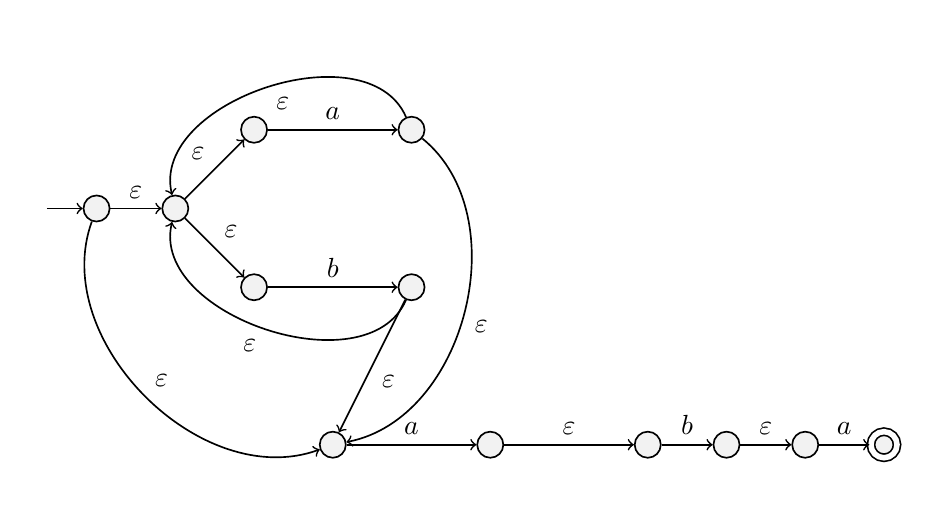
\begin{tikzpicture}
\tikzset{state/.style={circle,minimum width=8pt,draw,semithick,
fill=gray!10}}
\node[state , initial  ] (q0) at (0,0) {};
\node[state ] (q1) at (1,0) {};
\node[state ] (q2) at (2,1) {};
\node[state ] (q3) at (2,-1) {};
\node[state ] (q4) at (4,1) {};
\node[state ] (q5) at (4,-1) {};
\node[state ] (q6) at (3,-3) {};
\node[state ] (q7) at (5,-3) {};
\node[state ] (q8) at (7,-3) {};
\node[state ] (q9) at (8,-3) {};
\node[state ] (q10) at (9,-3) {};
\node[state , accepting ] (q11) at (10,-3) {};
\draw (q0) edge[] node {\tt $\epsilon$} (q1) ;
\draw (q1) edge[] node {\tt $\epsilon$} (q2) ;
\draw (q1) edge[] node {\tt $\epsilon$} (q3) ;
\draw (q2) edge[] node {\tt $a$} (q4) ;
\draw (q3) edge[] node {\tt $b$} (q5) ;
\draw (q4) edge[bend right = 85] node {\tt $\epsilon$} (q1) ;
\draw (q5) edge[bend left = 85] node {\tt $\epsilon$} (q1) ;
\draw (q6) edge[] node {\tt $a$} (q7) ;
\draw (q7) edge[] node {\tt $\epsilon$} (q8) ;
\draw (q8) edge[] node {\tt $b$} (q9) ;
\draw (q9) edge[] node {\tt $\epsilon$} (q10) ;
\draw (q10) edge[] node {\tt $a$} (q11) ;
\draw (q0) edge[bend right = 65] node {\tt $\epsilon$} (q6) ;
\draw (q4) edge[bend left = 65] node {\tt $\epsilon$} (q6) ;
\draw (q5) edge[] node {\tt $\epsilon$} (q6) ;
\end{tikzpicture}
\end{center}



\subsection{Lemma}

\begin{tcolorbox}
\begin{itemize}
	\item if a language is regular, then it is described by a regular expression .
\end{itemize}
\end{tcolorbox}



\section{Context-Free Grammars}

\textbf{context-free grammars} can describe certain features that have a recursive structure .

\noindent
Context-free grammars were first used in the study of human languages .

\noindent
an other important application of context-free grammars occurs in the application and compilation of programming languages .


\subsection{Context-Free Grammars Terms}

The following is an example of a context-free grammars  :

\begin{align*}
A &\to 0A1 \\
A &\to B \\
B &\to \# 
\end{align*}


\begin{itemize}
	\item a grammar consists of a collection of \textbf{substitution rules}, also called \textbf{productions}
	\item each symboled is called a \textbf{variable}
	\item The string consists of variables and \textbf{terminals}
	\item the variable often are represented by capital letter
	\item the terminals are in range of input alphabet and often represented by lowercase letters
	\item the sequence of substitutions to obtain a string is called a \textbf{derivation}
\end{itemize}


\begin{tcolorbox}
\begin{itemize}
	\item any language that can be generated by some context-free grammar is called a \textbf{context-free language (CFL)}
\end{itemize}
\end{tcolorbox}



\subsection{Formal Definition Of a Context-Free Grammar}

\begin{tcolorbox}
a \textbf{context-free grammar} is a 4-tuple $( V , \Sigma , R , S )$ , where :
\begin{itemize}
	\item $V$ is a finite set called the \textbf{variables}
	\item $\Sigma$ is a finite set, disjoint from $V$, called the \textbf{terminals}
	\item $R$ is a finite set of \textbf{rules},
	\item $S \in V$ is the start variable
\end{itemize}
\end{tcolorbox}


\begin{tcolorbox}
\begin{itemize}
	\item the \textbf{language of the grammar} is $\{ w \in \Sigma^{*} \: | \: S \xRightarrow{*} w \}$
\end{itemize}
\end{tcolorbox}


\subsection{Ambiguity}


if a grammar generates the same string in several different ways, we say that the string is derived \textbf{ambiguously} in that grammar . if a grammar generates some string \textbf{ambiguously}, we say that the grammar is \textbf{ambiguous}


\noindent
when we say that a grammar generates a string ambiguously, we mean that the string has two different parse trees, not two different derivations .


\begin{tcolorbox}
\begin{itemize}
	\item a string $w$ is derived \textbf{ambiguously} in context-free grammar $G$ if it has two or more different leftmost derivations . Grammar $G$ is \textbf{ambiguous} if it generates some string ambiguously .
\end{itemize}
\end{tcolorbox}


\newpage

\subsection{Chomsky Normal Form}
in context-free grammars, it is convenient to have them in simplified form . One of the simplest and most useful forms is called the \textbf{Chomsky Normal Form} . 


\begin{tcolorbox}
\begin{itemize}
	\item a context-free grammar is in \textbf{Chomsky Normal Form} if every rule is of the form :
	\begin{align*}
	A &\to BC \\
	A &\to a \\
	\end{align*}
	where $a$ is any terminal and A, B, and C are any variables | except that B and C may not be the start variable . in addition, we permit the rules $S \to \epsilon$, where $S$ is the start variable .
\end{itemize}
\end{tcolorbox}


\subsection{Theorem}

\begin{tcolorbox}
\begin{itemize}
	\item any context-free language is generated by a context-free grammar in Chomsky Normal Form .
\end{itemize}
\end{tcolorbox}



\newpage

\section{Push Down Automata}

PDA use different alphabet for its input and its stack , we specify input alphabet $\Sigma$ and a stack alphabet $\Gamma$ .

\noindent
Note that :
$\Sigma_{\epsilon} = \Sigma \cup \{ \epsilon \} $ and
$\Gamma_{\epsilon} = \Gamma \cup \{ \epsilon \} $ 




\begin{tcolorbox}
a \textbf{pushdown automaton} is a 6-tuple $( Q , \Sigma , \Gamma , \delta , q_{0} , F )$ , where $Q$ , $\Sigma$ , $\Gamma$ , and $F$ are all finite sets , and 
\begin{itemize}
	\item $Q$ is the set of states
	\item $\Sigma$ is the input alphabet
	\item $\Gamma$ is the stack alphabet
	\item $\delta :  Q \times \Sigma_{\epsilon} \times \Gamma_{\epsilon} \to P(Q \times \Gamma_{\epsilon})$ is the transition function
	\item $q_{0} \in Q$ is the start state
	\item $F \subseteq Q$ is the set of accept states
\end{itemize}
\end{tcolorbox}



\subsection{Theorm}

\begin{tcolorbox}
\begin{itemize}
	\item a language is context-free if and only if some pushdown automaton recognizes it .
\end{itemize}
\end{tcolorbox}



\subsection{Lemma}


\begin{tcolorbox}
\begin{itemize}
	\item if a language is context-free, then some push down automaton recognizes it .
\end{itemize}
\end{tcolorbox}



\subsection{Lemma}

\begin{tcolorbox}
\begin{itemize}
	\item if a pushdown automaton recognized some language, then it is context-free
\end{itemize}
\end{tcolorbox}


\newpage

\subsection{LR(k) grammar}

Algorithms for $LR(k)$ grammars introduce $lookahead$.

\noindent
The acronym LR(k) stands for : 
\begin{itemize}
	\item Left to right input processing
	\item Rightmost derivations( or equivalently, leftmost reductions )
	\item $k$ symbols of $lookahead$	
\end{itemize}



\begin{tcolorbox}
\begin{itemize}
	\item an \textbf{LR(k) grammar} is a context-free grammar such that the handle of every valid string is forced by lookahead $k$ .
\end{itemize}
\end{tcolorbox}




\section{Turing Machine}

The Turing machine model uses an infinite tape as its unlimited memory. It
has a tape head that can read and write symbols and move around on the tape.

\noindent
Initially the tape contains only the input string and is blank everywhere else. If
the machine needs to store information, it may write this information on the
tape. To read the information that it has written, the machine can move its
head back over it. The machine continues computing until it decides to produce
an output. The outputs accept and reject are obtained by entering designated
accepting and rejecting states. If it doesn’t enter an accepting or a rejecting state,
it will go on forever, never halting.

The following list summarizes the differences between finite automata and
Turing Machines .


\begin{enumerate}
	\item a Turing Machine can both write on the tape and read from it
	\item the read | write head can move both to the left and to the right 
	\item the tape is infinite
	\item the special states for rejecting and accepting take effect immediately
\end{enumerate}



\subsection{Formal Definition of a Turing Machine}

the heart of the definition of a Turing Machine is the transition function $\delta$ because it tells us how the machine gets from one step to the next . 

$$
\delta : Q \times \Gamma \to Q \times \Gamma \times \{ L , R \}
$$


when the machine is in certain state $q$ and the head is over a tape square containing a symbol $a$, and if $\delta(q,a) = (r,b,L)$, the machine writes the symbol $b$ replacing the $a$, and goes to the state $r$ . L or R indicates whether the head moves to the Left or Right after writing . In this case, the L indicates a move to the Left .



\begin{tcolorbox}
a \textbf{Turing Machine} is a 7-tuple $( Q , \Sigma , \Gamma , \delta , q_{0} , q_{accept} , q_{reject} )$ , where $Q , \Sigma , \Gamma $ are all finite sets
\begin{enumerate}
	\item $Q$ is teh set of states
	\item $\Sigma$ is the input alphabet not containing the \textbf{blank symbol}
	\item $\Gamma$ is the tape alphabet, where $b \in \Gamma$ and $\Sigma \subseteq \Gamma$
	\item $\delta : Q \times \Gamma \to Q \times \Gamma \times \{ L , R \}$ is the transition function
	\item $q_{0} \in Q$ is the start state
	\item $q_{accept} \in Q$ is the accept state 
	\item $q_{reject} \in Q$ is the reject state , where $q_{reject} \neq q_{accept} $
\end{enumerate}
\end{tcolorbox}



\begin{tcolorbox}
\begin{itemize}
	\item as a Turing Machine computes, changes occur in the current state, the current tape contents, and the current head location . a setting of these three items is called \textbf{configuration} of the Turing machine .
\end{itemize}
\end{tcolorbox}



\end{document}